\documentclass[border=10pt]{standalone}
  \usepackage{tikz}
  \usepackage{amsmath}
  \usetikzlibrary{arrows.meta, positioning, fit, backgrounds, calc}

  \begin{document}
  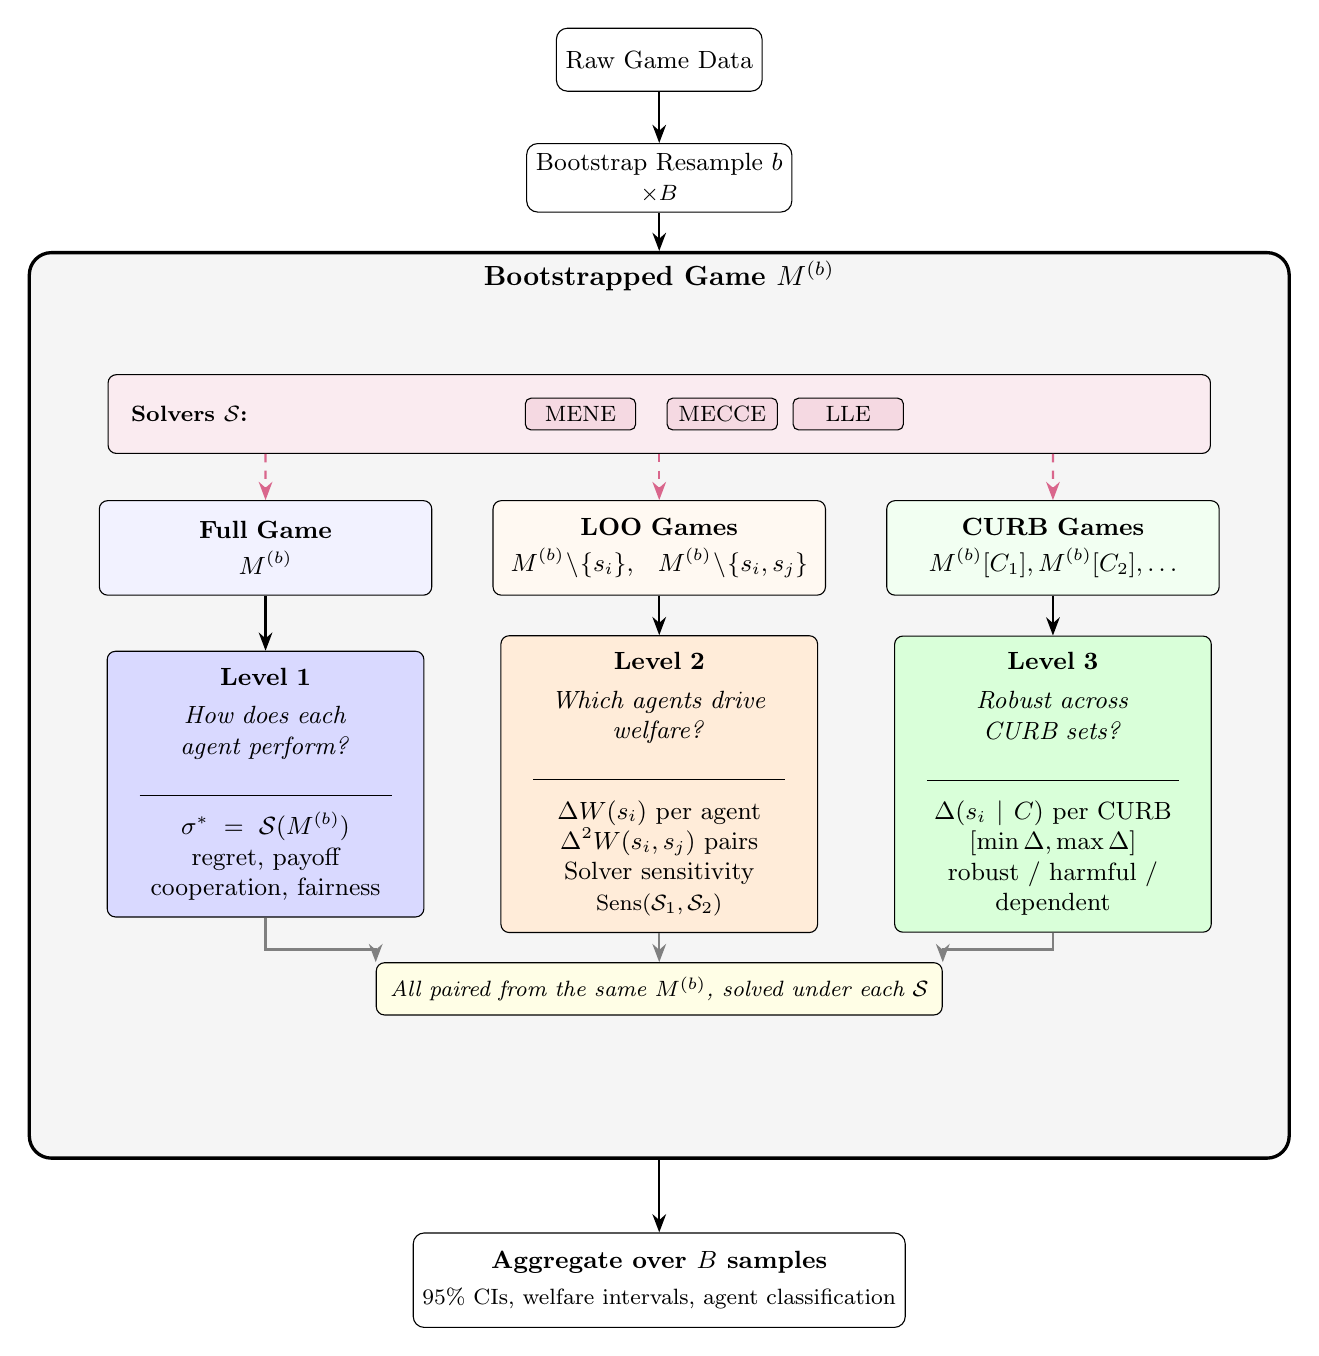
\begin{tikzpicture}[
      >=Stealth,
      font=\small,
      levelbox/.style={draw, rounded corners=3pt, minimum width=4cm, align=center, text width=3.6cm, inner sep=6pt},
      gamebox/.style={draw, rounded corners=3pt, minimum width=4cm, minimum height=1.2cm, align=center, text width=3.8cm, inner sep=6pt, fill=white},
      solverbox/.style={draw, rounded corners=2pt, minimum width=1.4cm, align=center, inner sep=3pt, font=\footnotesize},
      outerbox/.style={draw, very thick, rounded corners=8pt, inner sep=15pt, fill=gray!8},
      topbox/.style={draw, rounded corners=4pt, fill=white, minimum width=2.5cm, minimum height=0.8cm, align=center},
  ]

  % Raw data
  \node[topbox] (raw) at (0, 11) {Raw Game Data};

  % Bootstrap
  \node[topbox] (boot) at (0, 9.5) {Bootstrap Resample $b$ \\ {\footnotesize $\times B$}};

  \draw[->, thick] (raw) -- (boot);

  % Outer bootstrap box
  \node[outerbox, minimum width=16cm, minimum height=11.5cm] (outer) at (0, 2.8) {};
  \node[anchor=north, font=\bfseries] at (outer.north) {Bootstrapped Game $M^{(b)}$};

  % --- Solver bar ---
  \node[draw, rounded corners=3pt, fill=purple!8, minimum width=14cm, minimum height=1cm, inner sep=4pt] (solverbar) at (0, 6.5) {};
  \node[anchor=west, font=\bfseries\footnotesize] at ([xshift=5pt]solverbar.west) {Solvers $\mathcal{S}$:};
  \node[solverbox, fill=purple!15] (mene) at (-1, 6.5) {MENE};
  \node[solverbox, fill=purple!15] (mecce) at (0.8, 6.5) {MECCE};
  \node[solverbox, fill=purple!15] (lle) at (2.4, 6.5) {LLE};

  % --- Game boxes (all at same y) ---
  \def\gamey{4.8}
  \node[gamebox, fill=blue!5] (fullgame) at (-5, \gamey) {
      \textbf{Full Game} \\[2pt]
      $M^{(b)}$
  };
  \node[gamebox, fill=orange!5] (loogame) at (0, \gamey) {
      \textbf{LOO Games} \\[2pt]
      $M^{(b)} \!\setminus\! \{s_i\}$, \; $M^{(b)} \!\setminus\! \{s_i, s_j\}$
  };
  \node[gamebox, fill=green!5] (curbgame) at (5, \gamey) {
      \textbf{CURB Games} \\[2pt]
      $M^{(b)}[C_1], M^{(b)}[C_2], \ldots$
  };

  % --- Solver to game arrows: from solver bar bottom edge, straight down ---
  \draw[->, thick, dashed, purple!60] ([xshift=-5cm]solverbar.south) -- (fullgame.north);
  \draw[->, thick, dashed, purple!60] (solverbar.south) -- (loogame.north);
  \draw[->, thick, dashed, purple!60] ([xshift=5cm]solverbar.south) -- (curbgame.north);

  % --- Level boxes (all at same y) ---
  \def\levely{1.8}
  \node[levelbox, fill=blue!15] (L1) at (-5, \levely) {
      \textbf{Level 1} \\[3pt]
      \emph{How does each} \\
      \emph{agent perform?} \\[4pt]
      \rule{3.2cm}{0.4pt} \\[3pt]
      $\sigma^* = \mathcal{S}(M^{(b)})$ \\
      regret, payoff \\
      cooperation, fairness
  };
  \node[levelbox, fill=orange!15] (L2) at (0, \levely) {
      \textbf{Level 2} \\[3pt]
      \emph{Which agents drive} \\
      \emph{welfare?} \\[4pt]
      \rule{3.2cm}{0.4pt} \\[3pt]
      $\Delta W(s_i)$ per agent \\
      $\Delta^2 W(s_i, s_j)$ pairs \\
      Solver sensitivity \\
      {\footnotesize $\text{Sens}(\mathcal{S}_1, \mathcal{S}_2)$}
  };
  \node[levelbox, fill=green!15] (L3) at (5, \levely) {
      \textbf{Level 3} \\[3pt]
      \emph{Robust across} \\
      \emph{CURB sets?} \\[4pt]
      \rule{3.2cm}{0.4pt} \\[3pt]
      $\Delta(s_i \mid C)$ per CURB \\
      $[\min \Delta, \max \Delta]$ \\
      robust / harmful / \\
      dependent
  };

  % --- Game to level arrows ---
  \draw[->, thick] (fullgame.south) -- (L1.north);
  \draw[->, thick] (loogame.south) -- (L2.north);
  \draw[->, thick] (curbgame.south) -- (L3.north);

  % Arrow from bootstrap to outer box
  \draw[->, thick] (boot) -- (outer.north);

  % Paired annotation box
  \node[draw, rounded corners=3pt, fill=yellow!10, inner sep=5pt, font=\footnotesize\itshape] (paired) at (0, -0.8) {All paired from the same $M^{(b)}$, solved under each
  $\mathcal{S}$};

  % --- Level to paired arrows: all go straight down then converge ---
  \draw[->, thick, gray] (L1.south) -- (-5, -0.3) -| (paired.north west);
  \draw[->, thick, gray] (L2.south) -- (paired.north);
  \draw[->, thick, gray] (L3.south) -- (5, -0.3) -| (paired.north east);

  % --- Aggregate box — OUTSIDE the grey bootstrap box ---
  \node[draw, rounded corners=4pt, fill=white, minimum width=6cm, minimum height=1.2cm, align=center] (agg) at (0, -4.5) {
      \textbf{Aggregate over $B$ samples} \\[2pt]
      {\footnotesize 95\% CIs, welfare intervals, agent classification}
  };

  \draw[->, thick] (outer.south) -- (agg.north);

  \end{tikzpicture}
  \end{document}